
\subsection{Requirements}

\begin{itemize}
    \item \textit{Trustworthy / transparent:} While the concept of trust has been extensively explored as "having confidence in someone and believing they are good, sincere or honest"\footnote{https://www.oxfordlearnersdictionaries.com/definition/english/trust\_2}, the concept of trustworthy particularly in compuetr science is not uniformly defined. Several studies \cite{turstworthy_morality, turstworthy_privacy, trustworthy_perfomance} elaborate properties and requirements of trustworthy systems, from which we can identify repeating properties: reliable, correct and consistent over time performing of intended and expected functions in a secure manner. Furthermore, the properties can be extended to include preserving morality \cite{turstworthy_morality}, privacy \cite{turstworthy_privacy} or performance \cite{trustworthy_perfomance}. Even though preventing tampering and preserving privacy can be included into the definition of trustworthiness, we chose to distinct them, in order to emphasize their crucial roles in our model. By ensuring the system is trustworthy, stakeholders can confidently rely on the accuracy of compliance verification without needing to access sensitive data directly. Furthermore, transparency allows stakeholders to understand and examine the system and its processes, which promotes trust in the system.
    \item \textit{Tamper-proof / integrity:} Reflecting on insights from A, the system should operate reliably within a malicious model, where participants may behave deviant. As household might try to avoid meeting renewable energy standards, the model needs to ensure that privacy cannot be misused for tampering. Thus, the model is required to be designed in a way that makes any tampering evident, while still preserving the privacy of the household.
    \item Privacy-preserving 
    
\end{itemize}


\begin{figure*}[htb]
  \centering
  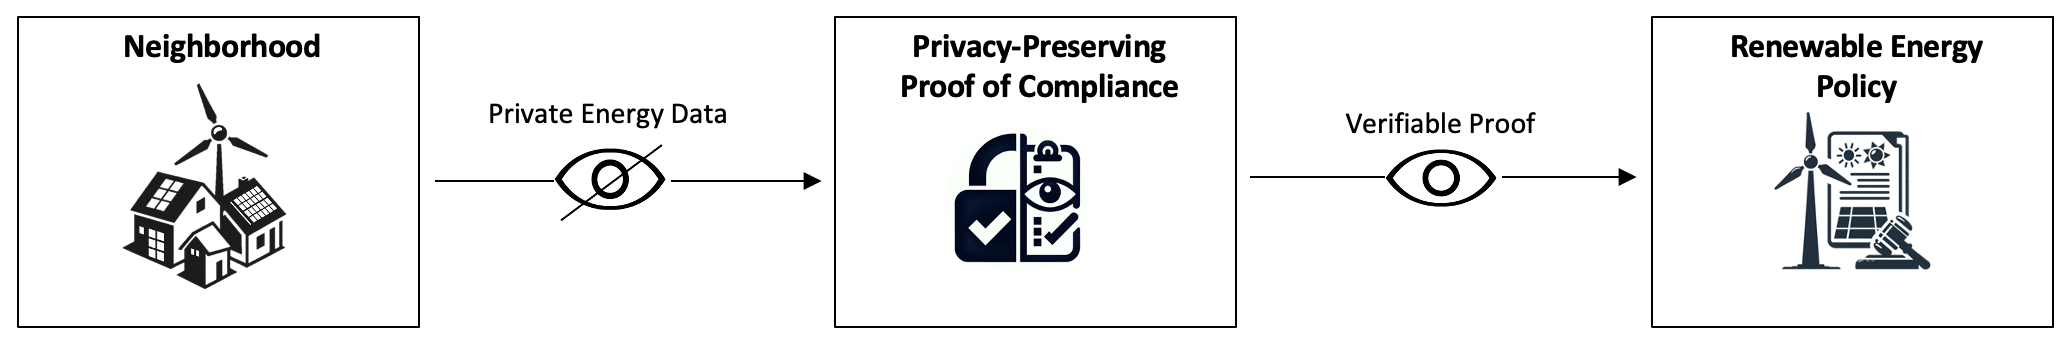
\includegraphics[width=1.5\columnwidth]{img/intro.png}
  \caption{Privacy-preserving verifiable proof of compliance for renewable energy consumption}\label{fig:intro}
\end{figure*}